%
% File: chap03.tex
% Author: Oliver J. H. Feighan
% Description: Theory and parameterization for chl-xTB method. 
% Include vibronic PES tests, and absorption spectra.
%
\let\textcircled=\pgftextcircled
\chapter{Chlorophyll specific methods}
\label{chap:chl_xtb}

\initial {T}his chapter reports the work done on designing and parameterising a
novel method for response properties. The framework and theory for the method is
outlined in section \ref{sec:theory}. Parameterisation details are given in 
section \ref{sec:chl_params}, including the reference data that compromised the 
training data, the objective function used and the algorithms that were used for
optimisation. The accuracy of this new method is showcased in the final section 
\ref{sec:chl_benchmarking}.

%=======
\section{Theory}
\label{sec:theory}

This section covers the approximations to full linear response theory that leads to the 
novel chl-xTB method. Starting from the eigenvalue equation, that is derived more
fully in the theory chapter but recapped here, a few key approximations lead to 
a framework that has tractable gradients and is less expensive than full linear
response. This fulfills the requirements set out in the introduction of having
an efficient and simple, but accurate, method of getting transition properties
for LHII chlorophylls.

\subsection{Full solutions TD-DFT equation}
In linear-response TD-DFT, excitation energies and characters are the solutions
of the non-Hermitian eigenvalue equation

\begin{equation}
    \begin{pmatrix}
        \mathbf{A}   & \mathbf{B} \\
        \mathbf{B}^\ast  & \mathbf{A}^\ast
    \end{pmatrix}
    \begin{pmatrix}
        \mathbf{X} \\
        \mathbf{Y}
    \end{pmatrix}
    = 
    \omega
    \begin{pmatrix}
        1 & 0 \\
        0 & -1
    \end{pmatrix}
    \begin{pmatrix}
        \mathbf{X} \\
        \mathbf{Y}
    \end{pmatrix}
\end{equation}
%
where $\mathbf{A}$, $\mathbf{B}$ are matrices whose elements describe the perturbation
of the electron density, the $\mathbf{X}$, $\mathbf{Y}$ solutions are the 
coefficients of excitations, similar to CIS, and eigenvalues $\omega$ are the 
excitation energies.

The elements of $\mathbf{A}$ and $\mathbf{B}$ correspond to descriptions of the
virtual-occupied and occupied-virtual contributions respectively, and in TD-DFT, 
with a global hybrid density functional, are given by

\begin{equation}
A_{ia,jb} = \delta_{ij} \delta_{ab} \left( \epsilon_a - \epsilon_i \right) + 2\left(ia|jb\right) - a_x\left(ij|ab\right) + (1- a_x)\left(ia|f_{\text{XC}}|jb\right)
\end{equation}
%
\begin{equation}
B_{ia,jb} = 2\left(ia|bj\right) - a_x\left(ib|aj\right) + (1- a_x)\left(ia|f_{\text{XC}}|bj\right)
\end{equation}
%
where indices $a,b$ and $i,j$ refer to virtual and occupied orbitals respectively,
$\epsilon_i$ is the orbital energy of orbtial $i$, $a_x$ is the value of non-local
Fock exchange in the XC functional $f_{\text{XC}}$. $\delta_{ij}$ is the Kronecker
delta function. The intergrals (here in Mulliken notation) can be seen to be of
Coloumb type for the $\mathbf{A}$ matrix and exchange for the $\mathbf{B}$ matrix. 
The leading term in the $\mathbf{A}$ matrix is the orbital energy difference,
which is contributes to the diagonal elements only due to the Kronecker deltas.

\subsection{Approximations to Solutions}
\label{subsec:chl_approxs}

There are three approximations made in the chl-xTB method. First is the Tamm-Dancoff 
approximation (TDA), which eliminates three blocks of the full linear response matrix.
Second is a diagonal dominant approximation to eigenvalue solutions, where diagonal 
elements of a matrix are taken as an approximation to true eigenvalues. The third
is a monopole approximation to two electron integrals which employs MNOK operators 
to accurately capture Coulomb and exchange functions. All these approximations 
reduce the amount of expensive electron integrals required to construct the full
eigenvalue equation, whilst still capturing the important aspects of the electron 
density response.

\subsubsection{Tamm-Dancoff approximation and Diagonal Dominant $\mathbf{A}$ matrices}
\label{subsubsec:Tamm_Dancoff}

One of the earliest approximations applied to full linear response was the Tamm-Dancoff
approximation, where only virtual-occupied contributions are calculated. This sets
all of the elements of $\mathbf{B}$ matrix to zero, and reduces the full eigenvalue 
equation to 

\begin{equation}
\mathbf{A} \mathbf{X} = \omega \mathbf{X}
\end{equation}
%
where the definitions of elements are the same as above, but it should be noted 
that the solutions $\mathbf{X}$ will be not be same. This is formally the same as
a CIS problem, and has been reported as a way to get back to CIS from full
TD-DFT.

As an eigenvalue problem, solving for $\omega$ requires constructing and diagonalising
the full $\mathbf{A}$ and then diagonlising. The XC functional is dependent on 
$\omega$ values and so several iterations of this diagonalisation are needed to
find stable, self-consistent solutions.

If the matrix is diagonal dominant, the diagonal elements of the $\mathbf{A}$ matrix 
can be used as an approximation to the eigenvalue solutions. This would be in the 
limit where the coupling elements (the off-diagonal elements) tend to zero, which
would be the case for an excitation that is mostly made up of a single transition.
Excitation energies would be given by

\begin{equation}
\omega_{ia} \approx A_{ia, ia} = \left( \epsilon_a - \epsilon_i \right) + 2\left(ia|ia\right) - a_x\left(ii|aa\right) + (1- a_x)\left(ia|f_{\text{XC}}|ia\right) 
\label{eq:diag_dom}
\end{equation}
%
. If the integrals are assumed to be small compared to the first term orbital energy
difference, then the orbital energy difference can be taken as an approximation 
to the full excitation energy, recovering the eigenvalue difference method from
the previous chapter.

By removing the eigenvalue problem, the gradients of the excitation energies are
more tractable. However the integral terms still require an interative, self-consistent
treatment. This can be simplified by using an approximation to these integrals that
uses point charge interactions.

It should be noted that further cost is removed by not needing to calculate not
only all of the off-diagonal elements but the diagonal elements for transitions
that are not of interest. This however would only be in the case where transitions
are not mixed. If transitions are mixed, then the coupling elements should be considered
and appproximating them to be zero would not be valid. This is considered in section
\ref{subsec:qy_transition}.

\subsection{Integrals approximations}
\label{subsec:MNOK}

The two electron integrals as written above are usually one of the most expensive
part of an electonic structure calculation. These can be approximated with a monopole
expansion, treating atomic sites as point charges, and using a charge-charge interaction 
for the energy.

Atom centered transition charges for transition $m \rightarrow n$ can be given in
the Mulliken scheme by summing the reduced one-electron transition density 
$\mathbf{D}^{mn}$ multiplied the orbital overlap $\mathbf{S}$ for all orbitals $p$ 
centred on atom $A$

\begin{equation}
q^{mn}_A = \sum_{p \in A} D^{mn}_{pq} S_{pq}  
\end{equation}
%
. Partial charges can be given as the difference between the electronic charge
and the nuclear charge $Z_A$

\begin{equation}
q_A = Z_A - \sum_{p \in A} D_{pq} S_{pq}  
\end{equation}
%
where $\mathbf{D}$ is the reduced one-electron density. This applies to any state,
so can be used to calculate ground state and excited state partial charges.

MNOK operators can recover the important behavior of full electron integrals that
is lost in classical charge-charge interaction, especially for the small distance limit.
For both coloumb and exchange type integrals, this can be done with a short-range
damped MNOK operators. The integral is approximated by

\begin{equation}
\left(pq|rs\right) \approx \frac{1}{2}\sum^N_A \sum^N_B q_A^{mm} q_B^{mn} \Gamma_{AB}
\end{equation}
%
where $N$ is the total number of atoms in the system and $p$,$q$,$r$, $s$ are electron
indices for both occupied and virtual orbitals. $A$ and $B$ are indices for the atoms.
For Coloumb type integrals, the operator $\Gamma_{AB}$ is given by

\begin{equation}
\Gamma^J_{AB} = \left(\frac{1}{\left(R_{AB}\right)^{y_J} + \left(a_x \eta\right)^{-y_J}} \right)^{\frac{1}{y_J}}
\end{equation}
%
where $R_{AB}$ is the interatomic distance and $\eta$ is the average of the chemical 
hardnesses. The chemical hardness of a given atom is defined as

\begin{equation}
\eta\left(A\right) = \frac{\delta^2 E\left(A\right)}{\delta^2 N^2}
\end{equation}
%
but in practice is precomputed and used as a static parameter. $y_J$ and $a_x$ are
global parameters, with the later used to recover the effects of Fock-exchange mixing
in the short-distance limit. For exchange type, the operator is

\begin{equation}
\Gamma^K_{AB} = \left(\frac{1}{\left(R_{AB}\right)^{y_K} + \eta^{-y_K}} \right)^{\frac{1}{y_K}}
\end{equation}
%
where the $y_K$ parameter replaces the $y_J$ parameter in the Coloumb type operator.

As the $a_x$ parameter can "mop up" many of the exchange effects, the density functional
in equation \ref{eq:diag_dom} is also neglected to further reduce computational cost.
The final form of the expression used to calculated excitation energies is then 
given by

\begin{equation}
\omega_{ia} = \left(\epsilon_a - \epsilon_i\right) + \sum^N_{A,B}\left(2 q_{ia}^A \Gamma^K_{AB} q_{ia}^B - q^A \Gamma^J_{AB} q^B\right)
\end{equation}
%
where the exchange term uses transition charges $q_{ia}$, and the Coloumb term uses
partial charges from the ground state density.

It can be seen that the inclusion of MNOK operators introduces global parameters
These would require optimisation to a training set. Initially it was investigated
whether parameterising to a training set with a broad range of systems and transitions
would be possible. However it was found that parameter optimisation procedures, 
whilst improving upon the accuracy of the \dxtb methods of the previous chapter,
could not break into the accuracy needed to investigate chlorophyll systems well
enough (discussed in more detail in \ref{subsec:ref_data}). This is due to many
transitions not being single character which would be not be consistent with the
diagonal dominant approximation. Additionally, the same issues as the previous 
chapter in assigning transition without symmetry made any autonomous optimisation
workflow difficult.

However a method that works for a wide set of systems is not required for LHII,
as only the \Qy transition is of interest for many models. Parameterising to a 
single, well-defined transition would be a much better approach for this investigation.
By reducing the scope of systems, the specificity of parameters can dramatically increase. 
This reduces the need to include more parameters to improve accuracy, as well as 
decreasing the amount of training data needed. Looking at other transitions and
systems then is outside the scope of this work, but could be a large area for further
work for similar investigations. An outline of the \Qy transition, and its applicability
to these approximations, is given below.

\subsection{\Qy Transition}
\label{subsec:qy_transition}
\begin{figure}
    \centering
    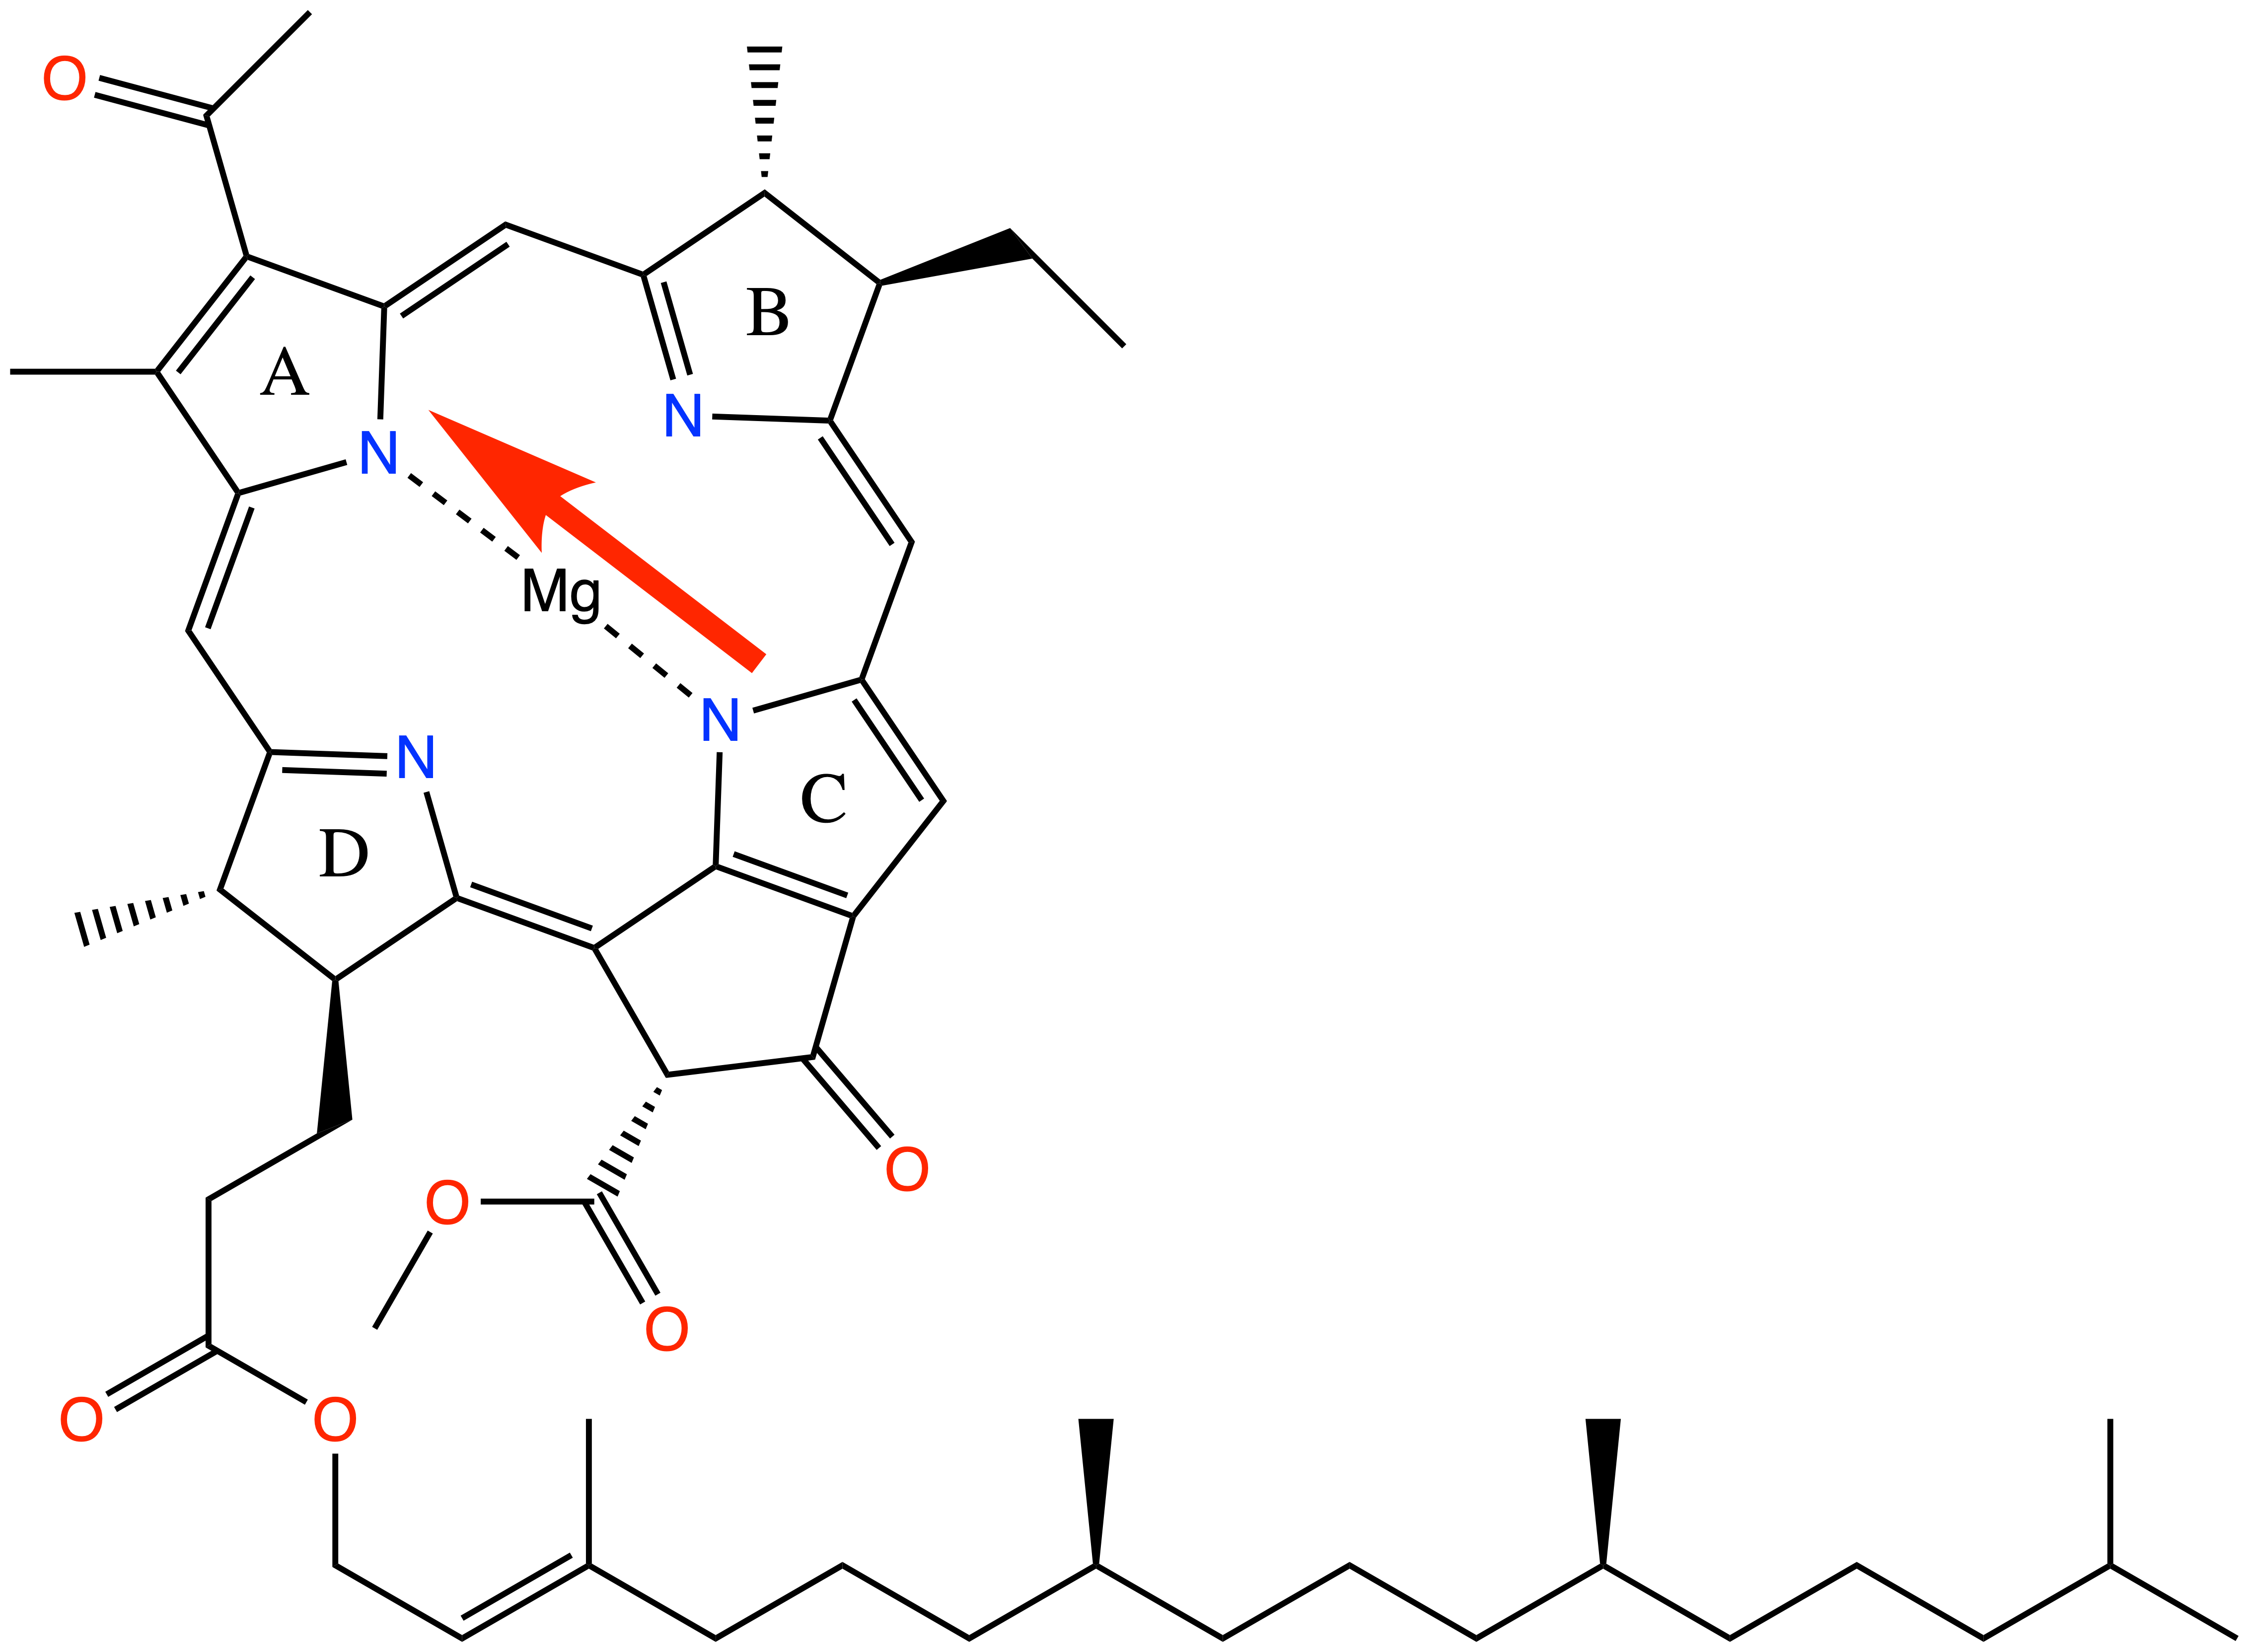
\includegraphics{chapters/chapter03/chlorophyll_Qy.png}
    \caption{Bacterial Chlorophyll a (BChla) with a model \Qy transition dipole.}
    \label{fig:bchla_qy}
\end{figure}

The \Qy transition is a good candidate to test approximations to full linear response 
theory. It is a well-defined transition which makes assignment easy, and has been
thoroughly analysed in the literature. It is also the most important transition 
in light harvesting systems, so an accurate treatment is necessary. 

The \Qy transition is the one of the two transitions that make up the $Q$ band in
the absorption spectra of chlorophyll, the other being the $Q_x$ transition. It 
is well known that the \Qy transition is important for electronic energy transfer,
and predicting both transition energies and transition dipole magnitudes and orientations
is important to construct frameworks for this transfer. The \Qy transition is mostly
HOMO-LUMO in character (~96\%), with a small amount of HOMO-1 - LUMO+1 (remaining 4\%).
The analogous transition in the unsubstituted tetraphorphyrin ring has the transition
dipole along the molecular axis defined by the N atoms, however due to the asymmetry 
introduced by substitutions and geometry deformations, this is usually not the case 
for BChla with a deviation from this axis of around 12 $^{\circ}$. The \Qy transition
in chlorophyll has its dipole component lying along the $N_A$-$N_C$ axis with $Q_x$ 
lying orthogonal, along the $N_B$-$N_D$ axis. $Q_x$ has the reverse character to 
the \Qy transition, being mostly HOMO-1 - LUMO+1.

Plots of the electron density of the HOMO and LUMO show how
this transition is delocalised over large sections of the porphyrin ring, with 
approximate $C_2$ symmetry along the molecular axes. Notable contributions can be
seen in the functional groups, giving the modified transition behaviour seen in 
different versions of chlorophyll, as well as the appearance of some features in
spectral density (discussed further in chapter \ref{chap:LHII}).

\begin{figure}
    \centering
    \includegraphics[scale=0.6]{../../Year_2/chlorophyll_parameterization/cube_files/HOMO_copy.png}
    \caption{The HOMO orbital of bacterial chlorophyll a from PBE0/Def2-SVP DFT.}
    \label{fig:HOMO}
\end{figure}

\begin{figure}
    \centering
    \includegraphics[scale=0.6]{../../Year_2/chlorophyll_parameterization/cube_files/LUMO_copy.png}
    \caption{The LUMO orbital of bacterial chlorophyll a from PBE0/Def2-SVP DFT.}
\end{figure}

It has recently also been shown that the high correlation between the eigenvalue
difference of HOMO-LUMO orbitals and full TD-DFT excitation energies implies that
the HOMO-1 - LUMO+1 transition can be excluded from the transition character. This
is also supported by the results for the chlorophyll test set in the previous chapter,
as \dscf with it's single transition treatment is able to capture \Qy transitions
with good accuracy.

The high amount of single-transition character in the \Qy transition makes it ideal
for the approximations to transition energies set out earlier. The lack of coupling
elements that would appear in the $\mathbf{A}$ matrix justifies both the use of
the diagonal dominant approximation and TDA. The almost exclusive centering of
electron density on main group elements make the use of MNOK integrals also valid.

Additionally, the well-defined transition make assignment trivial, and the transition
dipole orientation to the $N_A$-$N_C$ axis has been used as a metric for the accuracy
of transition dipole moments. As a single value, this is ideal for autonomous optimisation 
both for use in an objective function as well as for discarding outlier transitions.

The \Qy transition was then used to benchmark the novel response approximations.
The optimisation and construction of reference and training set data is discussed
later in section \ref{sec:chl_params}.

\subsection{Changes to xTB parameters}
\label{subsec:chl_method}

As found in the last chapter, the underlying electronic structure can have a huge
effect on the accuracy of transition properties, in some cases more than a change
in the response method. The xTB methods in particular, both linear response and
\dxtb, were particulary ill-suited for transition properties. Whilst DFT methods
could have been used as for Mulliken partial and transition charges, this would
still not be efficient enough to calculate the large volume of geometries from LHII. A 
tight-binding, semi-emperical approach for the electron structure is still required.
To improve the applicability of the xTB methods for transition properties, it was
decided that some of the parameters would need to be altered. A top-down approach
was used for these alterations, as it has been shown to work well for the GFN-xTB
and sTDA-xTB methods. 

As discussed in the theory chapter, the GFN1-xTB Fock matrix is made of both charge
depenedent and charge independent terms. The form of these terms, and definitions
of parameters, is also given in the theory chapter. Only the charge dependent terms would
have any effect on the partial and transition charges, thereby effecting the transition
properties. The charge dependent terms are the first, second and third density fluctuation
terms. The first order term is the leading term, and so parameters present in this
term were chosen to be included in the optimisation procedure to prioritise parameters
that would have the largest effect. Only some of these parameters are "free", 
whilst others are based on physical or \emph{ab initio} values. These are the H{\"u}ckel
parameters $k_l$, where $l$ is the angular momentum of the orbital, and the global
scaling parameters. The global scaling parameters are used to adjust interactions
for some pairs of elements where the global parameters led to incorrect bond lengths.
It was found that for the \Qy transition, only $Mg$ and $N$ interactions had to 
be scaled.

An obvious drawback of altering these parameters to fit to transition properties
is that they would lose their specificity to the GFN-xTB training set. However
it is not in the scope of this work to find a semi-empirical method that would be able
to calculate these properties for chlorophyll. chl-xTB is not used to calculate
optimised geometries or hessians of chlorophyll as other methods could be expected 
to perform better. Also if this were the necessary, including more target properties
in the parameter optimisation would decrease the accuracy to any one target, making
the method worse overall. For example, the sTDA-xTB and GFN-xTB methods use different
electronic structure parameters for this reason.

\subsection{Transition and Excited State Density from the Ground State}

Similar to \dscf, the ground state orbital coefficients are taken to be a good
approximation to the (\Qy) excited state coefficients. It was assumed then that
the excited state could be calculated without orbital relaxation, so that both the
excited state and ground state could be constructed from the same set of molecular
orbitals. The transition density is then calculated as

\begin{equation}
\mathbf{D}^{01} = \ket{\Psi^0} \bra{\Psi^1} 
\end{equation}
%
with $\bra{\Psi^0}$, $\bra{\Psi^1}$ (the ground and excited state respectively)
being constructed from the same set of molecular orbital coefficients $\mathbf{C}^0$
but with different sets of occupation numbers for the ground and excited state.
The ground state and excited state density can be similarly calculated as

\begin{equation}
\mathbf{D}^{0} = \ket{\Psi^0} \bra{\Psi^0}  
\end{equation}
%
\begin{equation}
\mathbf{D}^{1} = \ket{\Psi^1} \bra{\Psi^1}  
\end{equation}
%
. These density matrices are used to calculate the partial and transition charges
with the Mulliken scheme, which is in turn used to calculate the MNOK integrals.
The transition and molecular dipoles can be calculated as the trace of the dipole
operator with the density.

It should be noted the ground and excited states would be orthogonal in this scheme,
as they share the same set of MO coefficients. Additionally, only one cycle of the
SCC procedure would be necessary, which would eliminate the problem of convergence
in the \dscf excited state. It would also halve the computational time. Excited
state properties, such as the molecular dipole and partial charges can also be
calculated from the excited state density, which will be important for the exciton 
framework of the next chapter.

It was found, however, that transition dipoles calculated using this method were
much larger than TD-DFT. This was also observed for the \dscf and eigenvalue
difference methods, implying that the inclusion of the HOMO-1-LUMO+1 transition
is key to accurately describing the transition density. To recover this, an additional
parameter was included to scale the transition density, which both yielded the 
correct transition dipole magnitudes as well as drastically increasing the accuracy
of the method overall. This is discussed more in section \ref{subsec:ref_data}.

\afterpartskip
\section{Parameterization}
\label{sec:chl_params}
An objective function and algorithm is required to find minima in the parameter 
space, where the minima correspond to an optimised set of parameters. Reference data
to also required as a target. All of these elements are important for minimising
the amount of error in the final method, as well as determining how well chl-xTB
performs for different problems and other properties.

\subsection{Objective Function}
\label{subsec:obj_func}
At first, it would be argued that the root mean squared error (RMSE) to the reference 
transition energy should be the value that should be minimised, giving the objective
function as

\begin{equation}
f_{\text{RMSE}}\left(\mathbf{x}\right) = \sqrt{ \frac{1}{N} \sum^N_i \left( \Delta E_i  - \Delta E_{i, \text{ref.}}\right)^2}
\end{equation}
%
where $\textbf{x}$ is the set of parameters, $\delta E_i$, $\delta E_{i,\text{ref.}}$ 
are the transition energies for system $i$ from the chl-xTB method and reference
method respectively, $N$ is the number of systems used to calculated the objective
function value (these can be different when looking at training and testing sets).

However just using the RMSE has two issues. First is that other transition properties are not 
included in the optimisation, so the transition dipoles would be expected to have 
a large error. This can be fixed by including a metric for the error in transition dipoles.
The other issue is that a low RMSE does not guarantee a high correlation. A measure
of the correlation can be given by the coefficient of determination

\begin{equation}
R^2 = 1 - \frac{\sum^N_i \left(\hat{y}_i - y_i \right)^2}{\sum^N_i \left(\hat{y}_i - \bar{y}\right)^2}
\end{equation}
%
where $\hat{y}$, $y$ are the predicted and reference values, and $\bar{y}$ is the
average of the reference values. The correlation is a better metric for determining
if chl-xTB has a small enough random error to predict transition properties, however
it may not account for systematic errors. Both a low RMSE and high $R^2$ value are
needed to optimise fully to the reference data, and the two metrics are not mutually
inclusive.

By including both RMSE and $R^2$ values, for transition energies as well as dipole
magnitudes, the full objective function used was

\begin{equation}
f_{\text{full}} \left( \mathbf{x} \right) = \lambda_1 \text{RMSE} \left(\Delta E \right)+ \lambda_2 \text{RMSE}\left( \left| \mu \right| \right) + \lambda_3 \left(1 - R^2 \left( \Delta E \right)\right) + \lambda_4 \left( 1 - R^2 \left( \left| \mu \right| \right)\right)
\end{equation}
%
where $\lambda_n$ are weights necessary to keep all of the terms to a similar range.
This provides stability to the optimisation procedure, such that no one term dominates
the solution space.

\subsection{Minimisation Algorithms}
\label{subsec:algorithms}
Finding the optimal parameters for the chl-xTB method is a nonlinear problem. The
parameters so far stated can not be used to create a linear function that would
reproduce the value of the objective function. Therefore it's necessary to use
hueristics that can solve for these problems.

\subsubsection{Nelder-Mead}
\label{nelder_mead}
The Nelder-Mead method, as implemented in \code{SciPy}, is a modified version of a simplex
algorithm, that uses a $n$-dimensional shape to define a test region, and iteratively
searches the $n$-dimension space by reflecting the vertices of the test region. 
The test region, or more specifically the shape described by its vertices, is the
simplex. The simplex has $n+1$ vertices - for example, a 2-dimensional problem
would have a triangular simplex.
The algorithm starts with an initial simplex guess. It is important that the initial
guess covers enough area to avoid descending into any local minima, whilst not being
too large as to not take into account finer details of the parameter space.
The simplex is propagated by using a central value of the set of vertices, and using
this to either expand, contract or shrink the simplex, or reflect on of the vertices.
For example to find the parameters $\mathbf{x}$ that correspond to a minimum of
the function $f\left(\mathbf{x}\right)$

\begin{equation}
\min_{\mathbf{x} \in \mathbb{R}^n} f\left( \mathbf{x} \right)
\end{equation}
%
with initial simplex vertices $\mathbf{x}_1, \dots, \mathbf{x}_{n+1}$, the first 
step is to order the function values of the vertices

\begin{equation}
f\left(\mathbf{x}_1\right) \leq f\left(\mathbf{x}_2\right) \leq \dots \leq f\left(\mathbf{x}_{n+1}\right)
\end{equation}
%
and calculate the centroid of the set of vertices, excluding the worst vertex 
$\mathbf{x}_{n+1}$. The next steps then propagate the simplex, first by testing 
whether a reflection point $\mathbf{x}_r$ is better than the worst vertex used to
calculate the centroid

\begin{equation}
\mathbf{x}_r = \mathbf{x}_0 + \alpha\left(\mathbf{x}_0 - \mathbf{x}_{n+1}\right) 
\end{equation}
%
where $\mathbf{x}_0$ is the centroid point. There are then a set of three possibilities
for the value of $f\left(\mathbf{x}_r\right)$. First is that it the best value
found so far, and so the simplex should be expanded along the centroid-relfected 
vertex axis

\begin{equation}
\mathbf{x}_e = \mathbf{x}_0 + \gamma\left(\mathbf{x}_r - \mathbf{x}_0 \right).
\end{equation}
%
. The corresponding vertex of the two function values $f\left(\mathbf{x}_r\right)$, 
$f\left(\mathbf{x}_e\right)$ then replaces the "worst" vertex $\mathbf{x}_{n+1}$.

A second possibility is that the function value for the reflected vertex is better
than the worst vertex used to calculate the centroid, but worse than the best 
value, $f\left(\mathbf{x}_1\right) \leq f\left(\mathbf{x}_r\right) \leq f\left(\mathbf{x}_n\right)$.
In this case the $\mathbf{x}_{n+1}$ vertex is replaced by the reflected vertex.

The last possibility is that the reflected vertex has a greater function value than
any vertex used to calculate the centroid. In this case a new point (contraction),
or set of points (shrink) are used to propagate the simplex. Depending on whether
this function value is greater or less than the worst vertex in the simplex ($\mathbf{x}_{n+1}$),
the contracted point is either inside or outside of the simplex

\begin{equation}
    f\left(\mathbf{x}\right)= 
    \begin{cases}
    \mathbf{x}_c = \mathbf{x}_0 + \rho \left(\mathbf{x}_r - \mathbf{x}_0 \right)               & \text{if } f\left(\mathbf{x}_r\right) < f\left(\mathbf{x}_{n+1}\right)\\
    \mathbf{x}_c = \mathbf{x}_0 + \rho \left(\mathbf{x}_{n+1} - \mathbf{x}_0 \right)           & \text{otherwise } f\left(\mathbf{x}_r\right) \geq f\left(\mathbf{x}_{n+1}\right)
    \end{cases}
\end{equation}
%
if the contracted point $\mathbf{x}_c$ is give a smaller function value than the 
reflected point for the first case, or the worst point for the second case, it then
replaces the worst simplex vertex.

The final possibility is that both the contracted point function value is greater 
than either the reflected point or the worst point. In this case, the entire simplex
is shrunk around axes to the best vertex

\begin{equation}
\mathbf{x}_i = \mathbf{x}_1 + \sigma \left(\mathbf{x}_i - \mathbf{x}_1 \right)
\end{equation}

for $i \in \{1, \dots, n\}$.

Once either the worst vertex or all of the vertices are replaced, the new simplex
is used as the start of a further iteration. Iterations are stopped once a termination
criteria is met, such as a vertex function value being below a threshold.

Several versions of this method exist, that add additional constraints. This can
include keeping the volume of the simplex constant, which can promote a steepest
descent approach.

\subsubsection{Sequential Least-Squares Squadratic Programming}
\label{subsubsec:slsqp}
The SLSQP (Sequential Least-Squares Quadratic Programming) method is fundamentally
different to the previous Nelder-Mead method, and follows a quasi-Newton procedure
with additional factors to treat constraints.

The general problem is similar to Nelder-Mead, namely to solve

\begin{equation}
\min_{\mathbf{x} \in \mathbb{R}^n} f\left( \mathbf{x}\right)
\end{equation}

however with an arbitary amount of constraint functions $c$

\begin{equation}
c_i \left(\mathbf{x} \right) = 0
\end{equation}
\begin{equation}
c_j \left(\mathbf{x} \right) \leq 0
\end{equation}
%
where $i$, $j$ are indices of the constraint functions.
It is assumed that the space of $f$ and $c_n$ are one-to-one mappable on the
space of $x$, and also is continuously differentiable. Starting from an initial
value of $\mathbf{x}_0$, a search direction $d^k$ and step length $\alpha_k$ are
used to propagate the set of parameters by

\begin{equation}
\mathbf{x}_{k+1} = \mathbf{x}_k + \alpha_k \mathbf{d}_k
\end{equation}
%
. The search direction, analogous to the ratio of function value to gradient in 
the Newton-Raphson method, is calculated by solving the Lagrange function

\begin{equation}
\mathcal{L} \left(\mathbf{x}, \lambda\right) = f\left(\mathbf{x}\right) - \sum^m_n \lambda_n g_n \left( \mathbf{x}\right)
\end{equation}
%
with a quadratic approximation, that reduces the problem to a quadratic programming
subproblem

\begin{equation}
\min_d f\left(\mathbf{x}_k\right) + \nabla f\left(\mathbf{x}_k\right)^T d + \frac{1}{2}d^T \nabla^2_{xx} \mathcal{L} \left(\mathbf{x}_k, \lambda_k \right) d
\end{equation}
%
where the last term is often short-handed as the $\mathbf{B}$ matrix. This is the 
sequential quadratic programming method. A linear least squares subproblem could
be used instead of quadratic programming, which in would give the subproblem as

\begin{equation}
\min_d \left\| \left(\mathbf{D}_k\right)^{\frac{1}{2}} \left(\mathbf{L}_k\right)^T d + \left(\mathbf{D}_k\right)^{-\frac{1}{2}}\left(\mathbf{L}_k\right)^{-1}\nabla f \left(\mathbf{x}_k\right)\right\|
\end{equation}
%
where the matrices $\mathbf{L}$, $\mathbf{D}$ are from a diagonal decomposition 
of $\mathbf{B}$

\begin{equation}
\mathbf{L}_k \mathbf{D}_k \left(\mathbf{L}_k\right)^T = \mathbf{B}_k
\end{equation}
%
. With the solutions for $\mathbf{d}_k$ solved by these subproblems, the parameter vector
$\mathbf{x}$ can be propagated until similar termination criteria as the Nelder-Mead
method.

A visualisation finding a parameter set $\mathbf{x}$ corresponding to a local minimum
of the HimmelBlau function (a standard benchmark for optimisation algorithms) is
shown in figures \ref{fig:nelder_mead} and \ref{fig:slsqp}. The former shows the 
Nelder-Mead simplex vertices, with the latter showing iterations in the $\mathbf{x}$
space. It can be seen that the Nelder-Mead algorithm evaluates more points and covers
a broader space, whereas the SLSQP algorithm follows a more direct gradient descent. 

Both these methods were used to find optimal chl-xTB parameters, and it was found 
that the SLSQP method performed best, both in terms of the number of iterations,
stability, and in the overall value of the objective function. This could be due 
to the addition of contraints, however it is hard to say as the wrapping of \code{SciPy}
around the implementations of both methods make it a black-box that is hard to 
investigate further. The results of the optimisation is discussed in further detail
in section \ref{subsec:chl_opt_results}.

\begin{figure}
    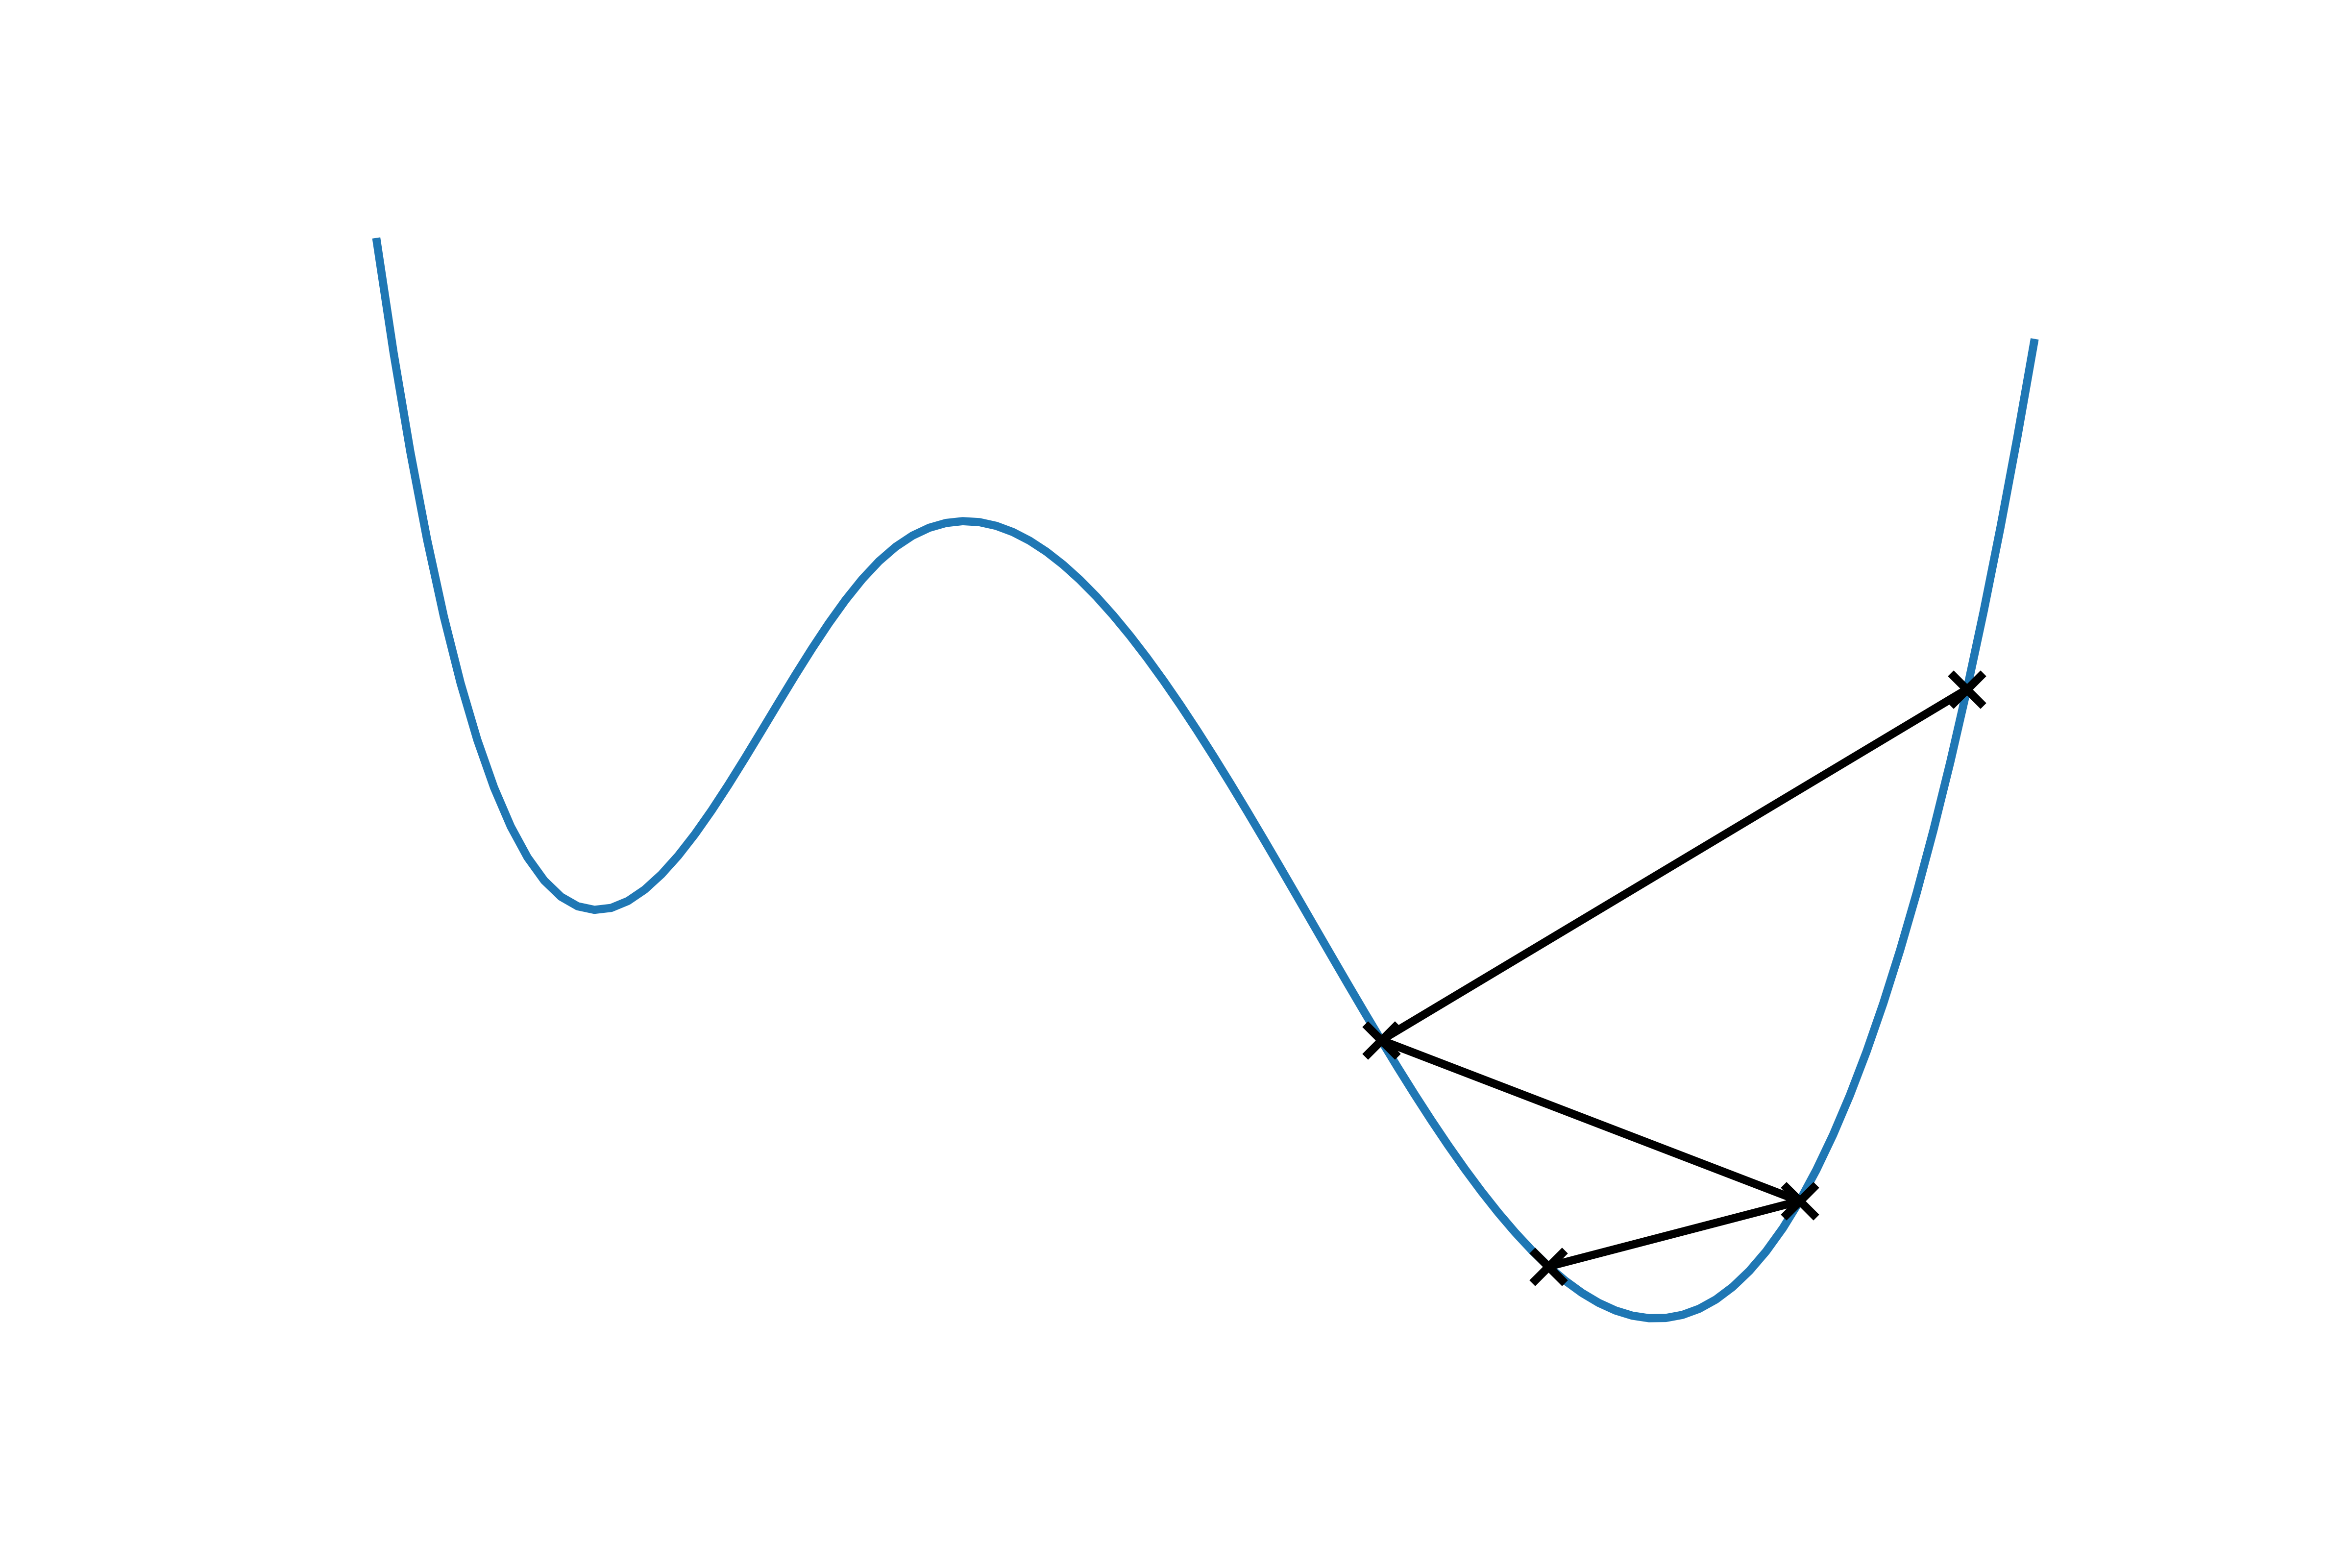
\includegraphics[scale=0.6]{nelder-mead.png}
    \caption{Positions of the Nelder-Mead simplex vertices for the HimmelBlau function.}
    \label{fig:nelder_mead}
\end{figure}

\begin{figure}
    \includegraphics[scale=0.6]{SLSQP.png}
    \caption{Positions of iterative solution vector $\mathbf{x}$ from SLSQP for
    the HimmelBlau funcion.}
    \label{fig:slsqp}
\end{figure}

\subsection{Reference Data}
\label{subsec:ref_data}
The geometries for the training set used to optimise the chl-xTB method were taken
from previously done molecular dynamics of the LHII protein \cite{Stross2016}. 
The geometries of LHII were chosen from uncorrelated snapshots, although each of
the 27 chlorophylls from each snapshot were included in the training data to account
for the differences in binding pockets. The stochastic collection of LHII snapshots
were chosen to cover a range of chlorophyll conformations to reduce the amount of
artificial bias towards any particular geometries.

Training the chl-xTB parameters was done against PBE0 data. This data was chosen
for the best accuracy-cost ratio, as well as having been previously used to investigate
exciton properties for the LHII system \cite{Stross2016}. Additionally, from the
outset it was unknown how much training data would be necessary, and so keeping 
potential future costs of expanding the training data down was another factor in 
choosing this functional.

\afterpartskip
\begin{table}
    \centering
    \begin{tabular}{|| c | c | c | c | c ||}
    \hline
                        & $\text{RMSE}\left(\Delta E\right)$ & $R^2\left(\Delta E\right)$ & $\text{RMSE}\left(\lvert \mu \rvert\right)$ & $R^2\left(\lvert \mu \rvert\right)$ \\
    \hline
    CAM-B3LYP           & 0.147 & 0.795 & 0.172 & 0.919 \\
    $\omega$-B97XD      & 0.200 & 0.650 & 0.214 & 0.876 \\
    BLYP                & 0.053 & 0.871 & 0.384 & 0.129 \\
    \dscf               & 0.225 & 0.847 & 1.455 & 0.566 \\
    $\Delta \epsilon$   & 0.218 & 0.875 & 1.511 & 0.500 \\
    ZINDO               & 0.596 & 0.339 & 1.526 & 0.396 \\
    \hline
    \end{tabular}
    \caption{ref data vals}
    \label{table:ref_data}
\end{table}

Transition properties were calculated with a range of methods, covering levels of
theory that would be comparable to the chl-xTB formalism. These included an eigenvalue
difference approach, \dscf, and TD-DFT with different levels of theory. This was
done so that the performance of any parameterisation results could be benchmarked
to an expected accuracy.

The errors and correlations of the reference data are shown in table \ref{table:ref_data}.
The methods included  in the benchmarking were \dscf, TD-DFT and eigenvalue difference
all using the PBE0 functional and Def2-SVP basis set. Also included are CAM-B3LYP
and BLYP functionals with Def2-SVP basis sets, as a higher and lower level reference
respectively. The basis set was not changed as it has been found that the basis
set has less importance on the accuracy than the functional \cite{Stross2016}.

There is a large variation in correlation and RMSE values for the reference methods
to PBE0. This variation sets a reasonable expectation of how well a new method
might perform.
The BLYP functional performs best with an RMSE of 0.053 eV, and is most correlated
(of the TD-DFT methods) with an $R^2$ value of 0.871. Second best is CAM-B3LYP,
with an RMSE of 0.147 eV. $\omega$-B97XD performs relatively well, with an RMSE
value of 0.200 eV, but has the lowest $R^2$ value of 0.650. This illustrates how
a low RMSE and high correlation are not mutually inclusive, and so must both be 
present in the objective function. 
The variance in these different TD-DFT methods, all of which have been used in studies
on chlorophyll, show how it is difficult to assign a true value to transition energy
for a set of geometries. Therefore as long as the accuracy of chl-xTB is within 
the range of methods shown here, it would also be valid.

The single transition methods also perform well, corroberating the earlier statement
that only treating a HOMO-LUMO transition can give accurate results. The \dscf and
eigenvalue difference methods have slightyl higher RMSE values, both around 0.22 eV.
However the correlation is much higher at of 0.847 and 0.875 a.u. respectively.
Hence, due to the dominance of HOMO-LUMO transition character, treating the transition
as mixed is not necessary in order to achieve accruacy for transition energies. 
The story for transition dipoles, however, is different.

The agreement of transition dipole magnitudes is much lower than excitation energies.
The RMSE of \dscf and eigenvalue difference methods is significantly higher (1.455
a.u. and 1.511 a.u. respectively) than the TD-DFT methods (0.172 a.u., 0.214 a.u.
and 0.384 a.u. for CAM-B3LYP, $\omega$-B97XD and BLYP respectively). The average
magnitude of PBE0 transition dipoles is 2.751 a.u., with the average for \dscf and 
eigenvalue difference being 4.287 a.u. and 4.342 a.u. respectively. This disparity
is attributed to the lack of inclusion of $Q_x$ transition character. As this dipole
component of this transition is orthogonal to \Qy, it may reduce the transition 
dipole magnitude similar to the effect seen in the outliers in the previous chapter.

Whilst there is a high degree of correlation between the higher level TD-DFT methods,
with 0.919 and 0.876 for CAM-B3LYP and $\omega$-B97XD respectively, the other methods
have a much lower correlation to PBE0 transition dipoles. BLYP is the worst correlated,
with a $R^2$ value of 0.129, which is fully uncorrelated. \dscf and eigenvalue difference
show a slight correlation at around 0.5.

Also included in the benchmarking was the semi-emperical method ZINDO. This had a
poor accuracy across the board, with RMSE and $R^2$ values of 0.596 eV and 0.339
for transition energies, and 1.526 a.u. and 0.396 for transition dipoles. It was
thought this might have good accuracy compared to TD-DFT and serve as a benchmark
for how well a semi-emperical method might perform, but this turned out to not be
the case.

Overall an RMSE to transition energies and dipoles of ~0.15 eV and ~0.2 a.u. is 
necessary to claim that transition properties can be calculated on a usable level 
of accuracy. Other cross-validations are necessary, and will be discussed in section
\ref{sec:chl_benchmarking}, but for the optimisation this provides a benchmark to 
aim for. Whilst a high correlation of around ~0.8 for both transition energies and
transition dipoles is possible, it can be seen that the latter may not be possible
for a single transition method.

\subsubsection{Training and testing set}
\label{subsubsec:train_test}
From the full set of PBE0 data, 100 random geometries were chosen for the training 
set and 507 geometries for the test set. The test set was used at the end of the 
optimisation procedure to validate how well the parameters perform on points outside 
of the training data. The sizes of each set was chosen to achieve a subset mean
error (how far the mean of the subset is from the full set of data) below 0.15 eV
for transition energies, whilst keeping a large number of geometries for the testing
set, as these are mutually exclusive.

\afterpartskip
\subsection{Results}
\label{subsec:chl_opt_results}

\begin{figure}
    \centering
    \includegraphics[scale=0.6]{../../Year_2/chlorophyll_parameterization/energy_training_scatter.png}
    \label{fig:energy_training_scatter}
    \caption{caption}
\end{figure}

\begin{figure}
    \centering
    \includegraphics[scale=0.6]{../../Year_2/chlorophyll_parameterization/dipole_training_scatter.png}
    \label{fig:dipole_training_scatter}
    \caption{caption}
\end{figure}

\begin{table}
    \centering
    \begin{tabular}{|| l r | r ||}
    \hline
    Hamiltonian & chl-xTB & GFN1/sTDA-xTB \\
    $k_\text{s}$ & 1.462 & 1.850 \\
    $k_\text{p}$ & 2.694 & 2.250 \\

    $\text{Mg}_\text{p}$ & 0.902 & - \\
    $\text{Mg}_\text{s}$ & 1.053 & - \\
    $\text{N}_\text{p}$ & 1.044 & - \\
    $\text{N}_\text{s}$ & 1.281 & - \\

    $\text{Mg}_\text{s}$-$\text{N}_\text{s}$ & 1.468 & - \\
    $\text{Mg}_\text{s}$-$\text{N}_\text{p}$ & 1.023 & - \\
    $\text{Mg}_\text{p}$-$\text{N}_\text{s}$ & 1.067 & - \\
    $\text{Mg}_\text{p}$-$\text{N}_\text{p}$ & 1.402 & - \\

    \hline\hline
    Response & & \\
    $y_K$ & 2.147 & 2.000 \\
    $y_J$ & 4.012 & 4.000 \\
    $a_x$ & 0.067 & 0.500 \\
    $D_{\text{scale}}$ & 0.636 & - \\
    \hline
    \end{tabular}
    \caption{optimized parameters from SLSQP procedure.}
    \label{table:chl_params}
\end{table}

Overall, the method performs extremely well considering the limitations as set out
above. Transition energies and dipole magnitudes are calculated well within acceptable
RMSE and correlation limits.

The final parameters for the chl-xTB method are given in table \ref{table:chl_params}.
The best performing set of parameters had an RMSE of excitation energy of 0.014 eV 
with an $R^2$ value of 0.88, and an RMSE of transition dipole magnitude of 0.057 a.u. 
with an $R^2$ value of 0.40. Repeated optimisation runs gave parameter and objective
function minima to similar values, and the difference in these values can be attributed
to the complex solution space. These values for RMSE are well within the values
for TD-DFT with various functionals, and the $R^2$ of transition energy is equally
good. While the correlation is low, it is near to the expected correlation from
\dscf and eigenvalue difference. It can also be seen in figure \ref{fig:dipole_training_scatter}
that the variation in chl-xTB transition dipole magnitude is much smaller than \dscf,
eigenvalue difference and ZINDO, as well as being close to the mean from PBE0. This
is a better behaviour, similar to the statiscal method used before \cite{Stross2016},
than the other methods with low correlations.

It was also found that lower minima of the objective function were found when using
the SLSQP method for optimisation instead of the default Nelder-Mead method. Minima
were found in a smaller number of iterations, reducing the overall CPU time required.
This is in line with benchmarked SLSQP solutions in a non-linear multidimensional space.
It was also investigated whether a reduction in the amount of parameters was possible,
by only training the response parameters and not the Hamiltonian parameters, however 
this did not achieve the same levels of accuracy as using both sets of parameters.

The initial guess for parameters were the corresponding GFN1-xTB and sTDA-xTB
parameters, or 1.0 for new parameters such as the Mg, N and transition density matrix
scaling.

The optimised values do not differ much from the original GFN1-xTB and sTDA-xTB
parameters (given for reference in table \ref{table:chl_params}), with the exception
of the $a_x$ parameter. This parameter is far lower than the sTDA-xTB equivalent,
which has a value of 0.500, but is in line with other methods that use similar MNOK
approximations for coulomb-type integrals in response methods \cite{Cho2021}.

\afterpartskip
\section{Cross-validation}
\label{sec:chl_benchmarking}

\subsection{Vibrational Mode Coupling}
\label{subsec:pot_energy_surfaces}

Whilst the stochastic selection of BChla geometries should represent a large section 
of the conformational space in LHII, it is not explicitly given that chl-xTB would
perform equally well along important vibrational modes. Explicitly testing the
values predicted by PBE0 and some of the reference methods as well as optimised
chl-xTB would show how well the geometry dependence has been "learnt". These values
would correspond to geometries that vary by a single normal mode displacement at 
a time to reduce error cancellation, as well as to show how well chl-xTB predicts
to the coupling of vibrational modes and transition properites.

The geometries for this test were not taken to be BChla for two reasons. There are
140 atoms in BChla, giving the number of normal modes is 414, and with ~10 coordinates
being calculated along each normal mode this represents a large number of geometries
that would require reference data with expensive functionals and basis sets. Additionally,
the normal modes would need to be calculated from an optimised geometry. The phytol
tail in BChla (and chlorophyll in general) make geometry optimisations difficult
due to the large degrees of freedom in rotations along the carbon chain. Without
an accuractely optimised geometry for the normal mode hessian, the predicted displacement
vectors for the normal modes would be useless.

Therefore the normal modes and transition properties were calculated for a truncated 
BChla with a hydrogen atom replacing the phytol tail, which made geometry optimisation
possible, and also reduced the total number of vibrational modes.

Normal modes with the strongest coupling to the \Qy transition were chosen to most
effectively scan the conformational space. These can be found by looking at modes
which break the symmetry of the \Qy transition. In an ideal model, the magnesium
and nitrogen centre have $D_{4h}$ symmetry with the \Qy transition lying along 
the $N_A$, $N_C$ axis. Vibrational modes with components along this axis will
therefore couple to the transition. The movement of $N_A$, $N_C$ atoms which induce
$D_{4h}$-$D_{2h}$ and $D_{4h}$-$C_{s}$ symmetry breaking are shown in figure \ref{fig:D4_sym_breaking}.

\begin{figure}[h]
    \centering
    
\includegraphics[scale=1.5]{chapters/chapter03/D4h_symmetry.png}
    \caption{Normal modes of the nitrogen-magnesium centre of chlorophyll that have
    $D_{4h}$-$D_{2h}$ (left) and $D_{4h}$-$C_{s}$ (right) symmetry breaking components.}
    \label{fig:D4_sym_breaking}
\end{figure}

Normal modes that would also have this symmetry breaking component were indentified
by how much the $N_A$-$N_C$ displacement would change along each normal mode. A plot of these
values, as well as the moving average, is shown in figure \ref{qy_length_scan}.
A similar scan was made of the $N_A$-$Mg$-$N_C$ angle, however less variance in
this value was found and the peak positions did not match previously reported frequencies
for strong coupling. Normal modes with the largest $N_A$-$N_C$ were then chosen 
for the transition properties scan.  It is interesting to note that the peaks in
the moving average line approximate the peaks in the chlorophyll \emph{a} absorption 
spectrum. The normal modes that were chosen had frequencies at 669.6, 701.7, 733.3,
745.5, 755.1, 1105.0, 1107.0, 1122.2, 1142.9, 1320.3, 1361.8 $\text{cm}_{-1}$, which
roughly correspond to previously indentified normal modes with frequencies of 728
and 1156 $\text{cm}^{-1}$ \cite{Kim2020}.

\begin{figure}
    \centering
    \includegraphics[scale=0.3, angle=90, origin=c]{../../Year_2/BChla_Qy/qy_length_scan.png}
    \label{fig:qy_length_scan}
    \caption{Change in the $N_A$-$N_C$ displacements along the set of GFN1-xTB 
    normal modes for a chlorophyll molecule truncated at the phytol tail.}
\end{figure}

\begin{figure}
    \centering
    \includegraphics[scale=0.3, angle=90, origin=c]{../../Year_2/BChla_Qy/qy_angle_scan.png}
    \label{fig:qy_angle_scan}
    \caption{Change in the $N_A$-$Mg$-$N_C$ angle along the set of GFN1-xTB normal
    modes for a chlorophyll molecule truncated at the phytol tail. The small smaller
    variance than in figure \ref{fig:qy_length_scan} led to this metric to not be
    used in normal mode choices.}
\end{figure}

For each selected normal mode, the geometry was propagated such that the sum of
all atomic displacements from the optimised geometry was in units of 1 $\AA{}$.
This was done up to 3 $\AA{}$ as it was found for most normal modes the energy 
difference between the optimised geometry and 3 $\AA{}$ displaced geometry was greater
than the thermal energy at 300 K. At each increment, the \Qy transtion energy and
dipole was calculated using chl-xTB, as well as TD-DFT with a PBE0/Def2-SVP level
of theory. Additionally, \dscf and the eigenvalue difference method was used as 
a benchmark, along with CAM-B3LYP TD-DFT with the same basis set. A quadratic
fit was also made for each of the methods and is shown in the plots. Some points
for the \dscf method are not shown as convergence for the excited state at these
geometries were not possible for similar reasons discussed in the previous chapter.

\begin{figure}
    \centering
    \includegraphics[scale=0.3]{../../Year_2/BChla_Qy/mode_83.png}
    \label{fig:mode_83}
\end{figure}

\begin{figure}
    \centering
    \includegraphics[scale=0.3]{../../Year_2/BChla_Qy/mode_85.png}
    \label{fig:mode_85}
\end{figure}

\begin{figure}
    \centering
    \includegraphics[scale=0.3]{../../Year_2/BChla_Qy/mode_88.png}
    \label{fig:mode_88}
\end{figure}

\begin{figure}
    \centering
    \includegraphics[scale=0.3]{../../Year_2/BChla_Qy/mode_90.png}
    \label{fig:mode_90}
\end{figure}

\begin{figure}
    \centering
    \includegraphics[scale=0.3]{../../Year_2/BChla_Qy/mode_91.png}
    \label{fig:mode_91}
\end{figure}

\begin{figure}
    \centering
    \includegraphics[scale=0.3]{../../Year_2/BChla_Qy/mode_129.png}
    \label{fig:mode_129}
\end{figure}

\begin{figure}
    \centering
    \includegraphics[scale=0.3]{../../Year_2/BChla_Qy/mode_130.png}
    \label{fig:mode_130}
\end{figure}

\begin{figure}
    \centering
    \includegraphics[scale=0.3]{../../Year_2/BChla_Qy/mode_132.png}
    \label{fig:mode_132}
\end{figure}

\begin{figure}
    \centering
    \includegraphics[scale=0.3]{../../Year_2/BChla_Qy/mode_135.png}
    \label{fig:mode_135}
    \caption{Transition energies and dipole magnitudes for the \Qy transition for
    geometries of truncated chlorophyll along normal modes, calculated with different
    response theories.}
\end{figure}

It can be seen that chl-xTB predicts PBE0 transition energies with a high degree
of accuracy. Transition dipole magnitudes are predicted with less good accuracy,
but still capture the main behaviour of PBE0 results well. chl-xTB consistently 
predicts PBE0 energies to within the same level of accuracy as achieved in the 
parameterisation test set. From the quadratic fits it can be seen that the gradients, 
turning points and curvature is well alligned between PBE0 and chl-xTB, especially
compared to \dscf and eigenvalue difference. It is also clear how important the
transition density scaling factor is in achieving accuracy for the transtion dipole
magnitudes, with \dscf and eigenvalue difference being well above where PBE0 and
CAM-B3LYP values sit.

It is argued that variations in chl-xTB transition properties, in addition to correctly
correlated with geometry variations, are also correctly correlated to the coupling
between normal modes and the \Qy transition. This is an important consideration 
for the later chapter on spectral density, where the assignment of spectral features
are based on comparison to vibrational modes.

\afterpartskip
\subsection{Absorption Spectra}
\label{subsec:absorption_spectra}

So far all of the benchmark and tests on chl-xTB have been for gas phase systems
and have no environmental effects. However in reality chlorophyll molecules would
be embedded in many different environments, for example the LHII protein. Although
the training set took structures that have been perturbed by the LHII protein, it
is important to test the behaviour of properties predicted by chl-xTB when explicitly
embedded. The obvious case for this would be predicting an absorption spectra for
chlorophyll when embedded by an explicit solvent. Additionally, it should be tested
whether the method could work for other chlorophyll systems other than Bchla. This
would be important for future investigations into chlorophyll systems, but for the
remaining work here it is not as important, and so isn't investigated fully.

The absorption spectra was calculated using frames from an MD trajectory of chlorophyll
A in an explicit diethyl ether solvent. An explicit solvent was used to account
for inhomogeneous broadening in the spectrum. The MD was performed with the
\code{OpenMM} toolkit. Forcefield parameters for the chlorophyll were taken from
a bespoke parameterisation for photosystem II \cite{Zhang2012}, with the rest of
the system using the OpenForceField. The structure for chlorophyll was taken from
the same source as the bespoke forcefield, and packed with explicit solvent using
the tools in the \code{Mistral} package. Equilibriation and production steps were 
done with a Langevin integrator set to 300 K  and a timestep of 0.5 femtoseconds.
The system energy was minimised before running a 10ps equilibriation. Frames were
then taken from a 2ns simulation time, with structures taken every picosecond.

Transition properties for chlorophyll structures from every frame were calculated.
This was done with the chl-xTB method, as well as PBE0 and CAM-B3LYP TD-DFT, both
using the Def2-SVP basis set. For the TD-DFT methods, the lowest excited state, 
rather than always the \Qy state, was taken for each frame, so as to fully capture 
the $Q$ band. Experimental data for the absorption spectra was also taken from Katz 
\emph{et. al} \cite{Strain1963}. Embedding effects were included in the chl-xTB
Fock matrix with a particle mesh Ewald method. The real space term was calculated
using \code{QCORE}, whereas the more complicated spline reciprocal space term was
calculated with the \code{HelPME} library. The absorption spectrum for each method
was calculated by a gaussian fit of a histogram of transition  energies. The fit
was normalised such that the area under all spectra matched that of the experimental 
spectrum. The absorption spectra, both with and without a single-parameter shift
of excitation energies, can be seen in \ref{fig:chl_diethyl_ether}.

\begin{figure}
    \centering
    \includegraphics[scale=0.4, angle=90, origin=c]{../../Year_2/AbsorptionSpectra/cla_diethyl_ether_spectra.png}
    \caption{Chlorophyll in diethyl ether.}
    \label{fig:chl_diethyl_ether}
\end{figure}

chl-xTB performs equally well as TD-DFT methods at simulating absorption spectra,
although constrained by the limits of the method and the training data.
It can be seen that the chl-xTB lineshape is similar in position and witdh to the
PBE0 method. This is highly encouraging, as the functional groups on chlorophyll A
can have a large effect on the \Qy transition, and so the good agreement here provides
evidence that important chemical features are still captured in different systems.
Although the chl-xTB lineshape is wider than the experimental spectrum, the CAM-B3LYP 
and PBE0 lines are also wider and so the chl-xTB is still within a reasonable expectation 
of accuracy.
Also seen is the lack of other peaks from the $Q$ band, which is present in the
experimental spectrum. The CAM-B3LYP data shows one peak at 510 nm, with PBE0 having
a very slight peak at around 380 nm. This is not present in the chl-xTB spectrum
as other $Q$ transitions are not calculated due to being outside of the training
data. The embedded chl-xTB spectra is both red-shifted and broadened slightly, which
is also observed in simulated spectra from other methods.

\section{Conclusions}
\label{sec:chl_conclusions}

It has been shown that novel approximations to the full linear-response eigenvalue
equation can give accurate predictions of transition properties from high-level methods.
This has been shown by optimising a set of parameters for the response approximations,
as well as for the underlying electronic structure.

Overall, chl-xTB performs as well as can be expected from the training data. Predictions
of transition energies and transition dipoles are incredibly close to the PBE0
values, and well within the error between different high level DFT functionals. 
The variations of these transition properties cab be attributed to geometry variations
rather than random error. 


From this it could be expected that improvements in the training data would yield 
better accuracy. This might be done by extending the training data in either the 
conformational space, or by investigating other systems. 

This was taken into consideration when investigating this method,
for example using CAM-B3LYP as training data instead of PBE0. This approach would
have two drawbacks. First would be that PBE0 has already been established for investigating
LHII properties, and so a clearer comparison of results for the exciton system would
be possible. Second is that a feature of this method is the reduced amount of 
computational cost required. If the amount of CAM-B3LYP data that may have been 
necessary to obtain increased too much then it would no longer be efficient to 
parameterise compared to using a different, lower level method. For other systems
smaller than chlorophyll, this might not be the case.
